% Einleitung
\section{Linear Block Codes}
A binary block code with $2^k$ code words of length $n$ is called a linear $(n,k)$ code, if and only if its $2^k$ 
code words form a $k$-dimensional subspace of the vector space of all the $n$-tuples over the field $\mathbb{F}_2$.\\

Definitions:\\
\begin{tabular}{| l |l | l |}
	\hline
	 block code			&	$(n,k)$				&	$n$: code symbols\\
						&						&	$k$: information symbols\\
						&						&	$n-k$: parity symbols \\
						&						&   $\hookrightarrow n-k$ check equations.\\
	\hline
	code word			&	$u=m \cdot G$ 		&	$u$: code word \\
						&						&   $m$: message \\
						&						&	$G$: generator matrix ($k \times n$-matrix).\\

	\hline
	Hamming weight:		&	$w(u)$				&	number of nonzero elements in u \\
						&						&	$w(101101b)=4$ \\
	minimum				&						& 	$w_{min}(C)=min\{w(u): u \in C, u \neq 0 \} $\\	
						&						&	$C$: a Code		\\		
	\hline	
	Hamming distance	&	$d(u,v)$			&	number of bit positions which $u$ and $v$ differ \\
						&						&	$d(101101, 001111)=2$ \\
						&	$d(u,v)=w(u+v)$		& \\
						&	$d(u,0)=w(u)$		& \\
						&	$d(u,v) \leq d(u,w) + d(w,v)$	& \\
	minimum				&						&	$d_{min}(C)=min\{d(u,v): u,v \in C, u \neq v \} $\\			
	\hline
	Error Detection		&	$\epsilon = d_{min}-1$ 		& $\epsilon$: number of detectable error bits \\
	Error Correction	&	$t=[\frac{d_{min}-1}{2}]$	& $t$: number of correctable error bits\\
	\hline
	Parity Check Matrix	&	$u \cdot H^T = \vec{0}$			& $H$: parity check matrix, $(n-k) \times n$-matrix\\
						&	$u \cdot H^T = m \cdot G \cdot H^T = \vec{0}$ & only for valid codeword $u$ \\
						&	$G \cdot H^T = \vec{0}$  \\
	\hline
	Syndrom testing		&	$s=r \cdot H^T$		&	$s$: syndrom \\
						&	$r = u + e$			&	$e$: error \\
						&						&	$r$: 'received' code word \\
						&						&	$s=0 \Rightarrow r$ is a valid code word \\
						&	$s(X)=r(X)\mod g(X)$	& $g(X)$: generator polynom \\
	\hline
	$P_{corr}$			&	$P_{corr}=\displaystyle\sum_{i=0}^{n} \alpha_i \cdot p^i \cdot (1-p)^{n-i}$		& $p$: bit error probability\\
	Prob. of correctly	&																					& $i$: Hamming weight of the pattern\\
	decoded vector		&																					& $\alpha$: number of pattern with the same Hamming weight\\
	\hline 
\end{tabular}\\
Hint: The minimum distance of a linear block code is equal to the minimum weight of its nonzero code words.\\

\subsection{Cyclic Codes}
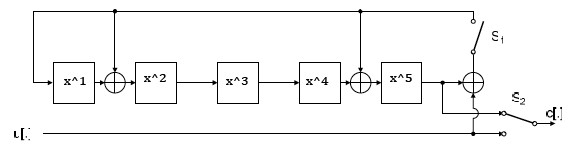
\includegraphics[width=11cm]{./bilder/shift_reg.png}
$\to$ \textbf{Polynom}: $g(x)=1+x^1+x^4+x^5$\\

\begin{list}{$\bullet$}{\setlength{\itemsep}{0cm} \setlength{\parsep}{0cm} \setlength{\topsep}{0.1cm}} 
\item Every cyclic shift of a code word is an other code word.
\item Two code words added give a new code word (so, 00..00 and 11..11 is often also a code word)
\item Generator Matrix $G$ are the linearly independent rows of the code word table.
\item Using Polynomials to represent a binary vector. \\
	  $u=(u_0, u_1,..u_{n-1}) \leftrightarrow u(X)=u_0 \cdot X^0 + u_1 \cdot X^1 + \ldots + u_{n-1} \cdot X^{n-1}$
\item Each code word $u$ corresponds to a polynomial $u(X)$ of degree $n-1$
\item In a $(n,k)$ cyclic code, there exists only one generator polynomial $g$ of degree $n-k$ with $g_0=1$
\end{list}

\subsubsection{Systematic Cyclic Codes (7,3)=(n,k)}
The code word $u$ must exhibit two properties:

\begin{list}{$\bullet$}{\setlength{\itemsep}{0cm} \setlength{\parsep}{0cm} \setlength{\topsep}{0.1cm}} 
  \item	It must be systematic: $u=(p_0,\ldots, p_{n-k-1}, m_0,\ldots,m_{k-1})$
  \item It must be a code word: $p(X)=X^{n-k}\cdot m(X) \mod g(X)$ \\
  \item $g(X)$ has the degree $n-k$ and must represent a valid code word
  \item The degree of $p(X)$ is always less than $n-k$
  \item $u=[p,m]$ (codeword)
  \item $s(X)=r(X)\mod g(X)$ (syndrom)
  \item $h(x)=X^n+1 : g(X)$ (check polynom)\\
        $H=\begin{bmatrix} 	
        			0	& \ldots	& \ldots	& 0 	& h_0		&	\ldots	&	h_m \\
        			0	& \ldots	& 0			& h_0	& \ldots	&	h_m		&	0	\\
        			\ldots &		&			&		&			&			&	\ldots \\
        			h_0	&	\ldots	& h_m		& 0		&	\ldots	&	\ldots	& 	0 \\
        \end{bmatrix}$  \\   
\end{list}
Achtung: in den Aufgaben ist LSB und MSB nicht wie gewohnt!\\

\subsubsection{Hamming Code}
$\alpha \to$ roots of the primitive polynomial.\\
\begin{list}{$\bullet$}{\setlength{\itemsep}{0cm} \setlength{\parsep}{0cm} \setlength{\topsep}{0.1cm}} 
  \item choose $m \geq 3$ (number of parity check equations)
  \item Length of code word $n=2^m-1$
  \item Length of message block $k=n-m$
  \item The Columns of the parity check matrix contain all integers between $1$ and $2^m-1$ as binary numbers. \\
		$H=[\ldots] $
  \item Every single bit error pattern yields a distinct syndrom vector
  \item checksum condition $\displaystyle\sum_{j=0}^{n-1}u_j \cdot \alpha^j = 0$
  \item where is the error:\\
  		$\displaystyle\sum_{j=0}^{n-1}r_j \cdot \alpha^j = \underbrace{\displaystyle\sum_{j=0}^{n-1}u_j \cdot \alpha^j}_{=0} + \underbrace{\displaystyle\sum_{j=0}^{n-1}e_j \cdot \alpha^j}_{=e_p \cdot \alpha^p}= \underbrace{\alpha^p}_{\text{error position}}$
  \item Parity check matrix: $H=[\alpha^0, \alpha^1, \ldots , \alpha^{n-1}]$

\end{list}

\subsubsection{BCH-Codes - Bose-Chaudhuri-Hocquenghem-Codes}
\begin{liste}
  \item choose a field $GF(2^m)$ for some positive integer m
  \item Let $\alpha$ be a primitive element of this field (root)
  \item A code word consists of $n=2^m-1$ binary digits. $u=(u_0, \ldots, u_{n-1})$
  \item Check sums $\displaystyle\sum_{i=0}^{n-1} u_i \cdot \alpha^{i \cdot q} = 0, \quad q=1,2,\ldots,r$
  \item This code can correct $t$ errors if $r \geq 2\cdot t-1$
  \item This code has $2^{n-rm}$ codewords
  \item even q are useless $\to \alpha=\alpha^2$ at $GF(2)$ $\to$ just evaluate the odd\\
     			$H=\begin{bmatrix} 	1 & \alpha   & \alpha^2     	& \ldots	& \alpha^{n-1} \\    		
   						   		1 & \alpha^3 & (\alpha^3)^2	& \ldots	& (\alpha^3)^{n-1}  \\    
   						   		1 & \alpha^5 & (\alpha^5)^2	& \ldots	& (\alpha^5)^{n-1}  \\   
   						   		\vdots	&	 &					&			& \vdots \\   						 
   						   		1 & \alpha^r & (\alpha^r)^2	& \ldots	& (\alpha^r)^{n-1}  \\   		
   			\end{bmatrix}$\\
			Note that the binary parity check matrix always starts with the LSB on top and MSB on bottom, e.g. $1=\begin{pmatrix} 1 \\ 0 \\ 0 \\ 0 \end{pmatrix}$ \\
\end{liste}

\textbf{Check if $u$ is valid codeword} \\
Variant 1:\\
If $u \cdot H^T = \vec{0}$, then $u$ is a valid codeword.\\

Variant 2 (not always applicable):\\
Example with $u=( 1 0 0 1 1 1 0 )\Rightarrow u(X)=1+X^3+X^4+X^5 \Rightarrow u(\alpha)=1+\alpha^2+1+\alpha^2+\alpha+1+\alpha+1=0 \Rightarrow u$ is a valid codeword. 

\subsection{RS Codes - Reed Solomon}
Reed-Salomon Codes are cyclic $(n, n-2t)$-Codes, which code symbols $u_i$ are not binary digits but elements of $GF(q)$. However, if $q=2^m$, then every code symbol
can be represented by a binary vector of length m. The number of correctable bits is given by $t$.\\


To build a systematic code with $k$-data symbols $(\bm m(X))$, $2t$ parity symbols and totally $k+2t=n$ symbols:
\begin{liste}
\item A primitive element $\alpha$ of $GF(2^m)$ has to be chosen. 
$\alpha$ is an element of order $2^m-1$: $\alpha^j\neq 1 \forall j\in [1,2^m-2]$; $\alpha^{2^m-1}=1$
\item The generator polynomial $\bm g(X)$ is:  $\bm g(X)=(X - \alpha^1) (X – \alpha^2)\ldots (X – \alpha^{2t})$
\item Calculate the parity symbols: $\bm p(X)=X^{n-k}\cdot \bm m(X) \mod \bm g(X)$
\item Sum up both together: $\bm u(X)=\bm p(X) +X^{n-k}\cdot \bm m(X) $
\item If the code word $\bm u(X) = u_0 + u_1 X+u_2 X^2\ldots+u_{n-1}X^{n-1} = ( u_0,  u_1, \ldots,  u_{n-1})$ is transformed into ``frequency space'', 
$U_k = \sum\limits_{i=0}^{n-1} u_i\cdot \alpha^{-i\cdot k}=\bm u(\alpha^{-k})$.
\item there have to be $2t$ zeros at the end of $\bm U=(U_0,U_1,\ldots,U_{k-1},0,\ldots,0)$
\end{liste}
e.g. (7,3)R-S code $(n=7, k=3 \Rightarrow 2t=4 \Rightarrow 2$ bit error correction$)$:
\begin{liste}
\item input: $\underbrace{010}_{\equiv a^1} \underbrace{110}_{\equiv a^3} \underbrace{111}_{\equiv a^5}$
\item input polynomial: $\bm m(X)=\alpha^1 + \alpha^3 X + \alpha^5 X^2$ 
\item The upshifted polynomial: $\bm m(X) X^{n-k}=\alpha^1 X^4 + \alpha^3 X^5 + \alpha^5 X^6$
\item calculate the parity polynomial: $\bm p(X)=\bm m(X) X^{n-k} \mod \bm g(X)\\
= \alpha^1 X^4 + \alpha^3 X^5 + \alpha^5 X^6 \mod \alpha^3 + \alpha^1 X + \alpha^0 X^2+\alpha^3 X^3+ X^4=\alpha^0+\alpha^2 X+\alpha^4 X^2 + \alpha^6 X^3$
\item $\bm u(X)=\alpha^0 + \alpha^2 X + \alpha^4 X^2 + \alpha^6 X^3+ \alpha^1 X^4 + \alpha^3 X^5 + \alpha^5 X^6$
\end{liste}
A correct code word is always a multiply of $\bm g(X)$ and has $2t$ zeros in the ``frequency space''. If not, this bit's represent the error pattern. 
To recalculate the \em error pattern \em the ``inverse DFT- inverse discrete fourier transformation'' 
$e_i(X)=\frac{1}{n}\sum\limits_{k=1}^n E_k(X) \alpha^{i \cdot k}=\bm E(\alpha^i)$ has to be used of the error pattern $\bm E= \bm R - \bm U$.\\
A less power intensive variant is the \em Berlekamp-Massey Algorithm \em. It finds the shortest linear feedback shift register which generate the 
whole error pattern out of the last $2t$ frequency symbols $R_{n-2t},\ldots,R_{n-1}$ (If there are less then t errors.).

\begin{minipage}{9cm}
\textbf{DFT-Matrix Representation}
$V=v \cdot A$\\
 $A=\begin{bmatrix} 	
    	\alpha^{-0\cdot 0}		& \alpha^{-0\cdot 1}		& 	\ldots	&\alpha^{-0\cdot (n-1)}	\\
    	\alpha^{-1\cdot 0}		& \alpha^{-1\cdot 1}		& 	\ldots	&\alpha^{-1\cdot (n-1)}	\\
    	\alpha^{-2\cdot 0}		& \alpha^{-2\cdot 1}		&	\ldots	&\alpha^{-2\cdot (n-1)}	\\
    	\vdots					&							&			& \vdots				\\
    	\alpha^{-(n-1)\cdot 0}	& \alpha^{-(n-1)\cdot 1}	&  	\ldots	&\alpha^{-(n-1)\cdot (n-1)}	\\
    \end{bmatrix}$  \\    
\end{minipage}
\begin{minipage}{9cm}
\textbf{IDFT-Matrix Representation}
$v=V \cdot A^{-1}$\\
 $A^{-1}=\frac{1}{n}\cdot \begin{bmatrix} 	
    	\alpha^{0\cdot 0}		& \alpha^{0\cdot 1}		& 	\ldots	&\alpha^{0\cdot (n-1)}	\\
    	\alpha^{1\cdot 0}		& \alpha^{1\cdot 1}		& 	\ldots	&\alpha^{1\cdot (n-1)}	\\
    	\vdots					&						&			& \vdots			\\
    	\alpha^{(n-1)\cdot 0}	& \alpha^{(n-1)\cdot 1}	&	\ldots	&\alpha^{(n-1)\cdot (n-1)}	\\
    \end{bmatrix}$  \\    
\end{minipage}\\
Define the dimension of the Matrix $A_{nxn}$ resp. of $A_{nxn}^{-1}$: $n = 2^m - 1 = q - 1$. Fill in the Matrix according to the above scheme and then 
calculate and simplify the exponent$\mod n$ (Example): $\alpha^{-4}=\alpha^2 \mod 3=\alpha + 1 \mod 3$. Note: $A \cdot A^{-1}=1$\\

\begin{minipage}{9cm}
	\textbf{Example of DFT calculation for Vector $v$}\\
	$V = v \cdot A = (1,\alpha,1+\alpha) \cdot \begin{bmatrix}
			1	&	1			&	1 \\
			1	&	1+\alpha	&	\alpha	\\
			1	&	\alpha		& 	1+\alpha \\
			\end{bmatrix}=(0,1,0)$
\end{minipage}
\begin{minipage}{9cm}		
	\textbf{Example of IDFT calculation for Vector $V$}\\
	$v = V \cdot A^{-1} = (0,1,0) \cdot \begin{bmatrix}
			1	&	1			&	1 \\
			1	&	\alpha		&	1+\alpha	\\
			1	&	1+\alpha	&	\alpha \\
			\end{bmatrix}=(1,\alpha,1+\alpha)$
\end{minipage}